\documentclass[a4paper,12pt]{article}

\title{Physics 30 \\ Electric Forces \& Fields}
\author{Jad Chehimi}

% document setup
\renewcommand{\familydefault}{\sfdefault}
\linespread{1.25}
\usepackage[margin=1in]{geometry}
\usepackage{setspace}
\usepackage{enumitem}
\setlist{nosep}
\usepackage{color,soul}
\setcounter{secnumdepth}{0}

% tools
\usepackage[hidelinks]{hyperref}
\usepackage{float}
%% images
\usepackage{graphicx}
\graphicspath{ {./images/} }
%% science
\usepackage{siunitx}
\sisetup{exponent-product=\times, per-mode=fraction}

\begin{document}
\maketitle

% temp
\begin{center}
\Huge
Unfinished!
\normalsize
\end{center}
% temp

\tableofcontents

\pagebreak

\section{Electric Fields}
\subsection{Micheal Faraday}
\begin{itemize}
    \item{Developed the idea of "lines of force" to describe electric fields}
    \item{A field is a \hl{"sphere of influence"} in which a force can affect an object at a distance \hl{without contact}}
    \item{There are electric, gravitational, and magnetic fields}
    \item{The symbol for electric field is $|\vec{E}|$}
\end{itemize}

\subsection{Gravitational Fields}
\Large $$\vec{g} = \SI{9.81}{\m\per\s\squared}$$ \normalsize

\Large $$\vec{g} = \frac{Gm}{r^2}$$ \normalsize
\begin{itemize}
    \item{$G$ = gravitational constant ($\SI{6.67e-11}{\N\cdot\m\squared\per\kg\squared}$)}
    \item{$m$ = mass of planet}
    \item{$r$ = radius of the planet}
\end{itemize}

\pagebreak
\section{Drawing Electric Field Lines}
\begin{figure}[H]
    \centering
    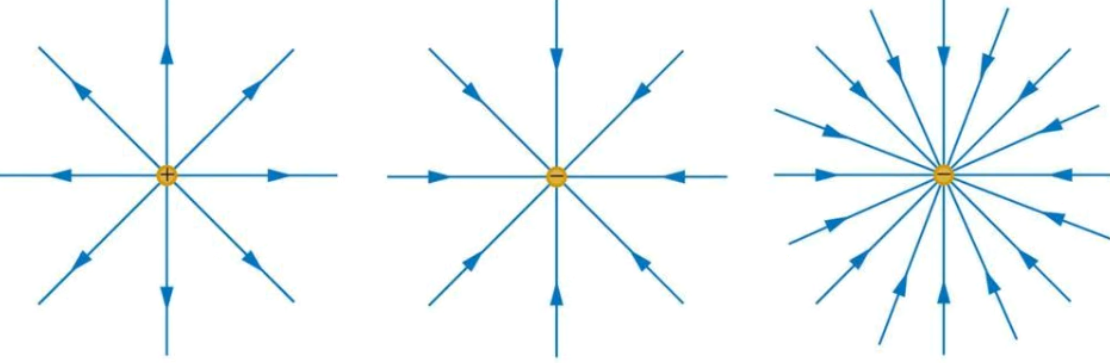
\includegraphics[width=0.75\textwidth]{fieldlines}
\end{figure}
\begin{itemize}
    \item{Like charges repel, opposite charges attract}
    \item{The field is stronger the closer to the source charge it is}
    \item{We \textbf{always} use a \hl{small positive test charge} to map/draw the electric field}
\end{itemize}

\subsection{Rules}
\begin{itemize}
    \item{The lines must originate on a positive charge and end on a negative charge (\hl{positive to negative})}
    \item{The electric field line must be \hl{perpendicular to the surface} of the charge}
    \item{The \hl{number of lines} drawn leaving a positive charge or approaching a negative charge is proportional to the \hl{magnitude of the charge}}
    \item{\hl{No two field lines can cross} each other}
\end{itemize}

\subsection{Electric Field Around A Positive v/s Negative Source Charge}
\begin{figure}[H]
    \centering
    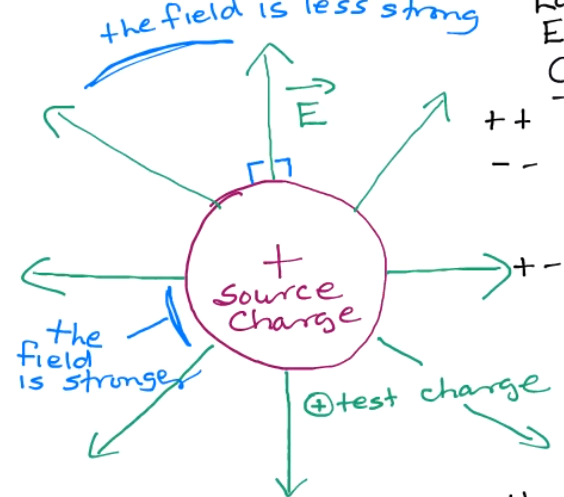
\includegraphics[width=0.4\textwidth]{lines}
    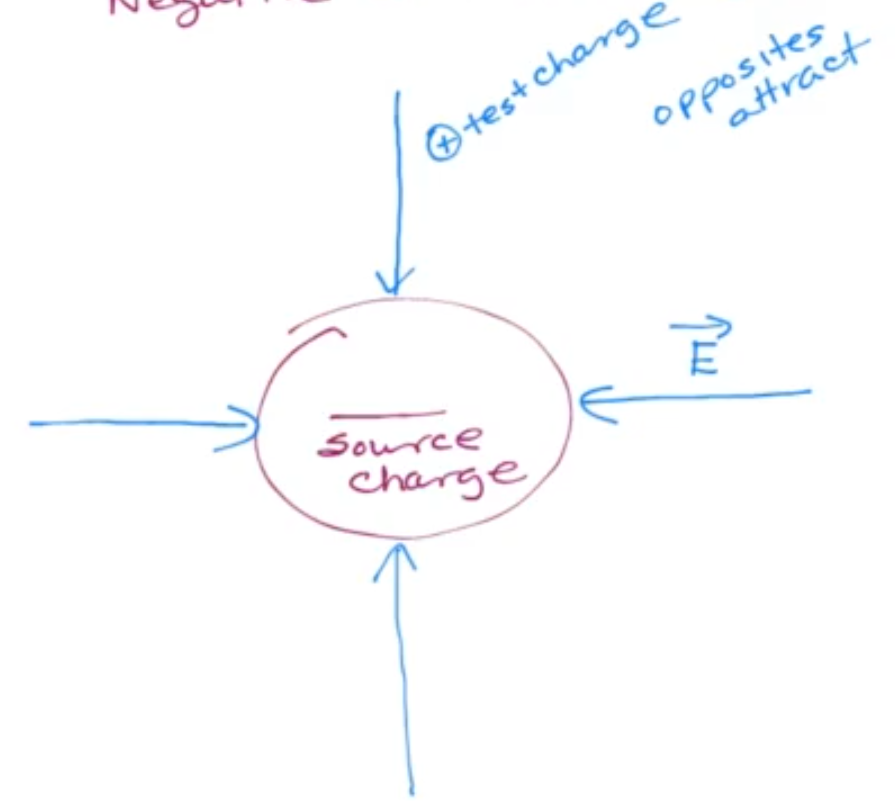
\includegraphics[width=0.4\textwidth]{lines2}
\end{figure}

\subsection{Electric Field Interactions}
\begin{figure}[H]
    \centering
    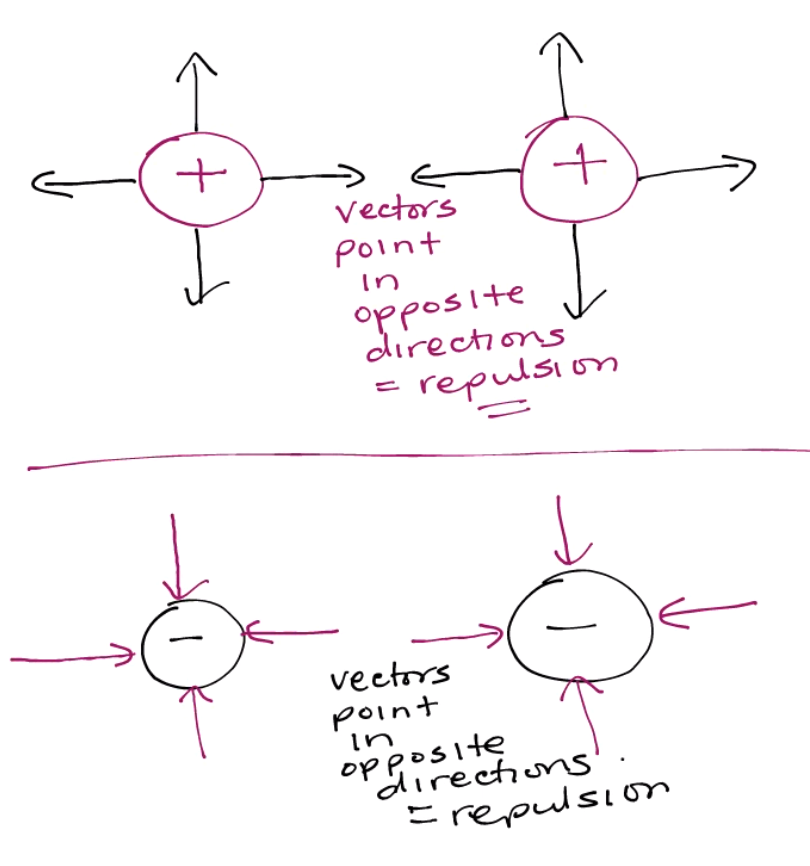
\includegraphics[width=0.4\textwidth]{repel}
    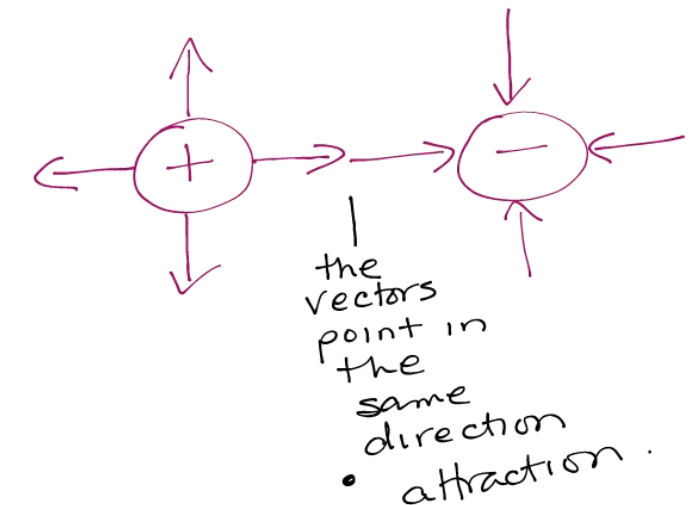
\includegraphics[width=0.4\textwidth]{attract}
\end{figure}

Use this theory with a test particle to determine the direction of an electric field. NOT signs.

\section{Particles}
\begin{figure}[H]
    \centering
    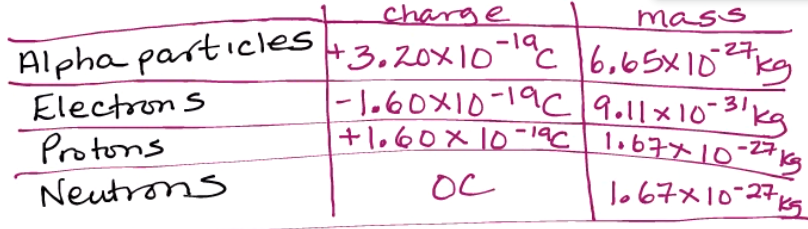
\includegraphics[width=\textwidth]{particles}
\end{figure}

\section{Electric Field Strength}
\subsection{Electric Field Around A Producer (Source Charge)}
\Large $$|\vec{E}| = \frac{kq}{r^2}$$ \normalsize
$$\textrm{Units: } \si{\newton\per\coulomb} \textrm{ or } \si{\V\per\m}$$
\begin{itemize}
    \item{$k$ = Coulomb's Constant (\SI{8.99e9}{\newton\cdot\m\squared\per\coulomb\squared})}
    \item{$q$ = Value of the source charge (\si{\coulomb})}
    \item{$r$ = Distance from the source charge (\si{\m})}
\end{itemize}

\subsection{Electric Field Experienced By A Charge}
\Large $$\vec{E} = \frac{\vec{F}_e}{q}$$ \normalsize
\begin{itemize}
    \item{$\vec{E}$ = Electric Field (\si{\newton\per\coulomb})}
    \item{$\vec{F}_e$ = Electrostatic Force (\si{\newton})}
    \item{$q$ = Test Charge (in a field question, its not source charge) (\si{\coulomb})}
\end{itemize}

\subsection{Example}
Calculate the electric field \SI{2.00}{\cm} from an alpha particle.
$$|\vec{E}| = \frac{(\SI{8.99e9}{\newton\cdot\m\squared\per\coulomb\squared})(\SI{3.20e-19}{\coulomb})}{(\SI{2.00e-2}{\m})^2}$$
$$|\vec{E}| = \SI{7.19e-6}{\newton\per\coulomb} \textrm{ radially outward}$$
\begin{figure}[H]
    \centering
    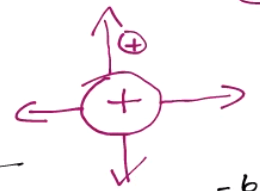
\includegraphics[width=0.3\textwidth]{fieldquestion}
\end{figure}

\subsection{Example II}
Calculate the electric field strength at a point in space where a \SI{3.24e-6}{\coulomb} charge experiences an electrostatic force of \SI{5.29e-3}{\newton}.
$$\vec{E} = \frac{\vec{F}_e}{q}$$
$$\vec{E} = \frac{\SI{5.29e-3}{\newton}}{\SI{3.24e-6}{\coulomb}}$$
$$\vec{E} = \SI{1.63e3}{\newton\per\coulomb}$$

\pagebreak
\subsection{Example III}
Calculate the electric field midway between the two charges below if they are \SI{5.00}{\cm} apart.
\begin{figure}[H]
    \centering
    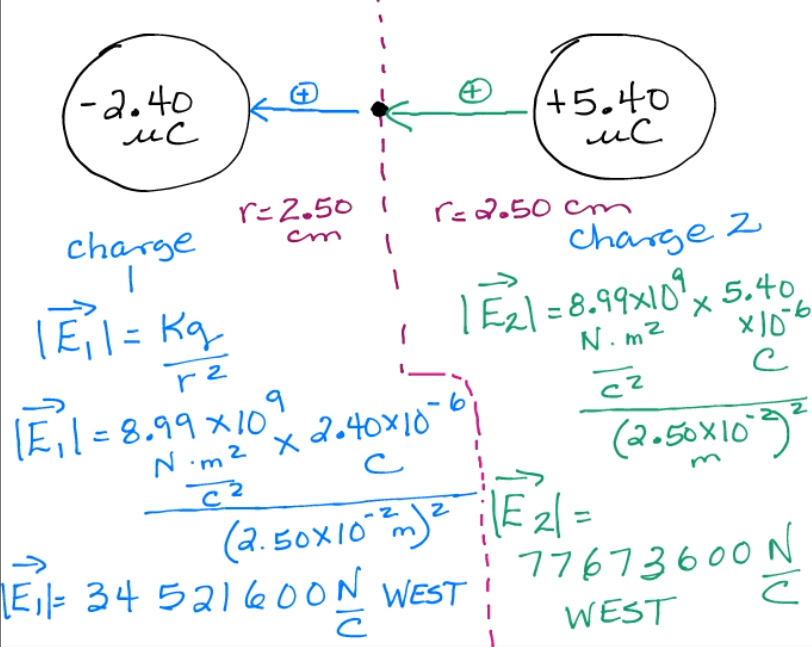
\includegraphics[width=\textwidth]{fieldquestion3}
\end{figure}

$$|\vec{E}_{net}| = |\vec{E}_1| + |\vec{E}_2|$$
$$|\vec{E}_{net}| = \SI{34521600}{\newton\per\coulomb}\textrm{, west} + \SI{77673600}{\newton\per\coulomb}\textrm{, west}$$
$$|\vec{E}_{net}| = \SI{1.12e8}{\newton\per\coulomb}\textrm{, west}$$

\pagebreak
\subsection{Electric Field Around A Producer in Two Dimensions}
\begin{itemize}
    \item{Calculate $\vec{E}$ of the hypotenuse}
    \item{Use trig to get the components of the electric field vector on each side}
\item{
    Direction of the vector is determined by the source charge like before
        \begin{itemize}
            \item{if positive, towards test charge/point (repel)}
            \item{if negative, from test charge/point to source charge (attract)}
        \end{itemize}
    }
    \item{Add the $x$ and $y$ components, positive or negative depending on direction}
    \item{You are left with the components of the net electric field vector}
\end{itemize}

\subsubsection{Example I}
\begin{figure}[H]
    \centering
    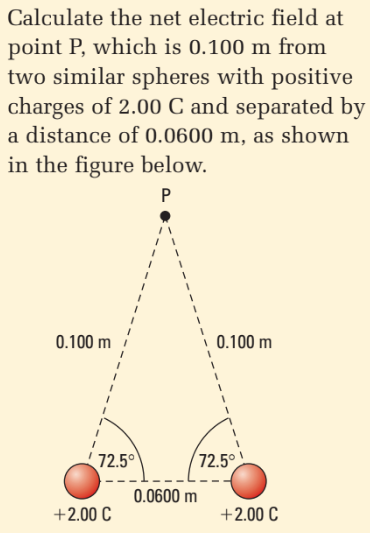
\includegraphics[width=0.3\textwidth]{fieldtriangle}
\end{figure}
$$= \SI{3.43e12}{\newton\per\coulomb}$$

\pagebreak
\section{Electric Field Between Plates}
\Large $$\vec{E} = \frac{V}{d}$$ \normalsize
\begin{itemize}
    \item{$V$ = total voltage across the plate (\si{\volt})}
    \item{$d$ = total distance between the plates (\si{\meter})}
\end{itemize}

\begin{figure}[H]
    \centering
    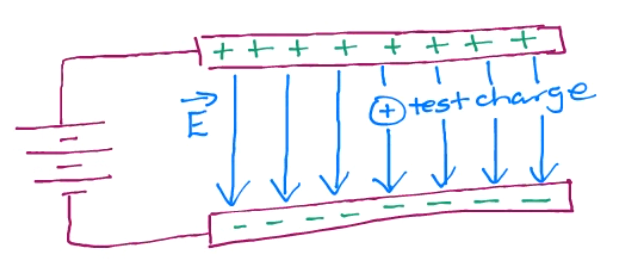
\includegraphics[width=0.50\textwidth]{plate}
\end{figure}

\begin{itemize}
    \item{The electric field between \hl{charged parallel plates} is \hl{uniform} --- identical at any point}
    \item{To determine the \hl{direction} of the electrical field between charged parallel plates, use a \hl{small positive test charge}}
    \item{
        Don't forget that \hl{work is equal to $\SI{0}{\joule}$} if the $F_e$ and $d$ are \hl{not along the same line}
        \begin{itemize}
            \item{$\theta$ (in $W = Fd\cos{\theta}$) must be either\\\ang{0} (force and distance same direction) or \\\ang{180} (force and distance opposite directions)}
        \end{itemize}
    }
\end{itemize}

\subsection{Example}
Two parallel plates are connected to a \SI{12.0}{\volt} battery. If the plates are \SI{6.00e-2}{\m} apart, calculate the electric field strength between them.
$$\vec{E} = \frac{\SI{12.0}{\volt}}{\SI{6.00e-2}{\m}} = \SI{200}{\volt\per\m}$$

\subsection{Example II}
\begin{figure}[H]
    \centering
    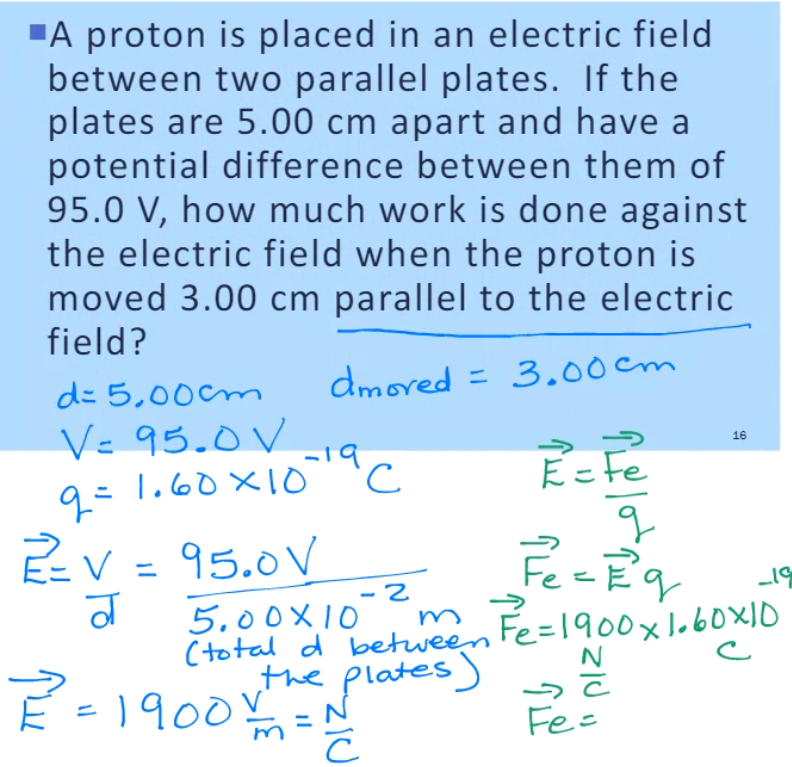
\includegraphics[width=0.45\textwidth]{workplate1}
    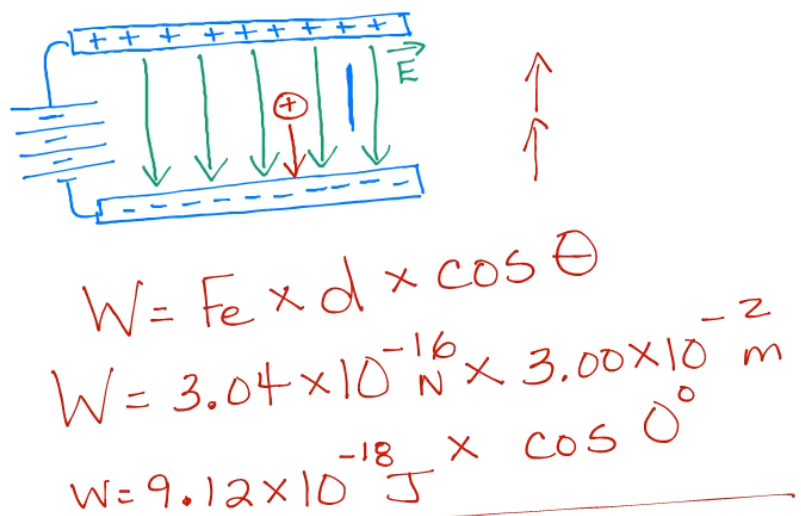
\includegraphics[width=0.45\textwidth]{workplate2}
\end{figure}

\section{Electric Field as a Function of r Graph}
\begin{itemize}
    \item{Make sure all values are times ten to the power of the same exponent before you plot}
\end{itemize}

\begin{figure}[H]
    \centering
    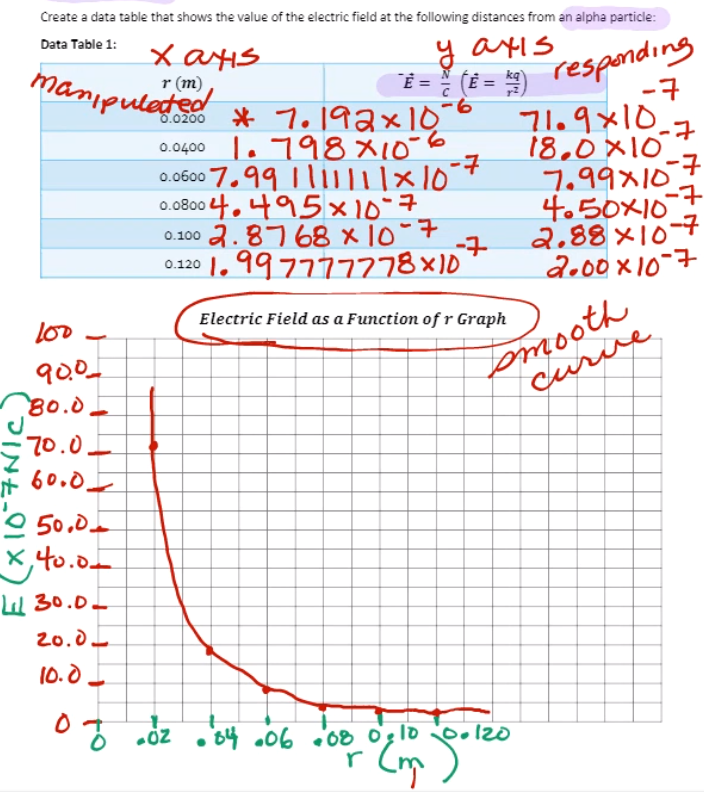
\includegraphics[width=0.75\textwidth]{graph1}
\end{figure}

In order to get a graph that is a straight line, set the $x$ to whatever is proportional to $y$. In this case, $E \propto \frac{1}{r^2}$

\begin{figure}[H]
    \centering
    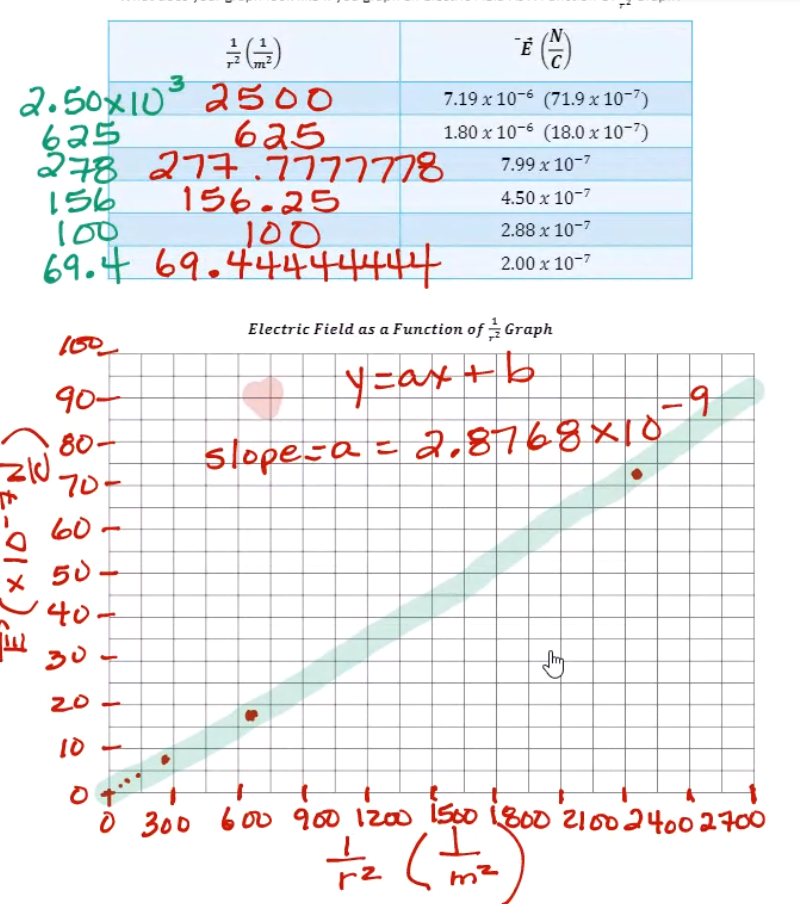
\includegraphics[width=0.75\textwidth]{graph2}
\end{figure}

\end{document}
